% Options for packages loaded elsewhere
\PassOptionsToPackage{unicode}{hyperref}
\PassOptionsToPackage{hyphens}{url}
%
\documentclass[
]{article}
\usepackage{amsmath,amssymb}
\usepackage{lmodern}
\usepackage{iftex}
\ifPDFTeX
  \usepackage[T1]{fontenc}
  \usepackage[utf8]{inputenc}
  \usepackage{textcomp} % provide euro and other symbols
\else % if luatex or xetex
  \usepackage{unicode-math}
  \defaultfontfeatures{Scale=MatchLowercase}
  \defaultfontfeatures[\rmfamily]{Ligatures=TeX,Scale=1}
\fi
% Use upquote if available, for straight quotes in verbatim environments
\IfFileExists{upquote.sty}{\usepackage{upquote}}{}
\IfFileExists{microtype.sty}{% use microtype if available
  \usepackage[]{microtype}
  \UseMicrotypeSet[protrusion]{basicmath} % disable protrusion for tt fonts
}{}
\makeatletter
\@ifundefined{KOMAClassName}{% if non-KOMA class
  \IfFileExists{parskip.sty}{%
    \usepackage{parskip}
  }{% else
    \setlength{\parindent}{0pt}
    \setlength{\parskip}{6pt plus 2pt minus 1pt}}
}{% if KOMA class
  \KOMAoptions{parskip=half}}
\makeatother
\usepackage{xcolor}
\usepackage[margin=1in]{geometry}
\usepackage{color}
\usepackage{fancyvrb}
\newcommand{\VerbBar}{|}
\newcommand{\VERB}{\Verb[commandchars=\\\{\}]}
\DefineVerbatimEnvironment{Highlighting}{Verbatim}{commandchars=\\\{\}}
% Add ',fontsize=\small' for more characters per line
\usepackage{framed}
\definecolor{shadecolor}{RGB}{248,248,248}
\newenvironment{Shaded}{\begin{snugshade}}{\end{snugshade}}
\newcommand{\AlertTok}[1]{\textcolor[rgb]{0.94,0.16,0.16}{#1}}
\newcommand{\AnnotationTok}[1]{\textcolor[rgb]{0.56,0.35,0.01}{\textbf{\textit{#1}}}}
\newcommand{\AttributeTok}[1]{\textcolor[rgb]{0.77,0.63,0.00}{#1}}
\newcommand{\BaseNTok}[1]{\textcolor[rgb]{0.00,0.00,0.81}{#1}}
\newcommand{\BuiltInTok}[1]{#1}
\newcommand{\CharTok}[1]{\textcolor[rgb]{0.31,0.60,0.02}{#1}}
\newcommand{\CommentTok}[1]{\textcolor[rgb]{0.56,0.35,0.01}{\textit{#1}}}
\newcommand{\CommentVarTok}[1]{\textcolor[rgb]{0.56,0.35,0.01}{\textbf{\textit{#1}}}}
\newcommand{\ConstantTok}[1]{\textcolor[rgb]{0.00,0.00,0.00}{#1}}
\newcommand{\ControlFlowTok}[1]{\textcolor[rgb]{0.13,0.29,0.53}{\textbf{#1}}}
\newcommand{\DataTypeTok}[1]{\textcolor[rgb]{0.13,0.29,0.53}{#1}}
\newcommand{\DecValTok}[1]{\textcolor[rgb]{0.00,0.00,0.81}{#1}}
\newcommand{\DocumentationTok}[1]{\textcolor[rgb]{0.56,0.35,0.01}{\textbf{\textit{#1}}}}
\newcommand{\ErrorTok}[1]{\textcolor[rgb]{0.64,0.00,0.00}{\textbf{#1}}}
\newcommand{\ExtensionTok}[1]{#1}
\newcommand{\FloatTok}[1]{\textcolor[rgb]{0.00,0.00,0.81}{#1}}
\newcommand{\FunctionTok}[1]{\textcolor[rgb]{0.00,0.00,0.00}{#1}}
\newcommand{\ImportTok}[1]{#1}
\newcommand{\InformationTok}[1]{\textcolor[rgb]{0.56,0.35,0.01}{\textbf{\textit{#1}}}}
\newcommand{\KeywordTok}[1]{\textcolor[rgb]{0.13,0.29,0.53}{\textbf{#1}}}
\newcommand{\NormalTok}[1]{#1}
\newcommand{\OperatorTok}[1]{\textcolor[rgb]{0.81,0.36,0.00}{\textbf{#1}}}
\newcommand{\OtherTok}[1]{\textcolor[rgb]{0.56,0.35,0.01}{#1}}
\newcommand{\PreprocessorTok}[1]{\textcolor[rgb]{0.56,0.35,0.01}{\textit{#1}}}
\newcommand{\RegionMarkerTok}[1]{#1}
\newcommand{\SpecialCharTok}[1]{\textcolor[rgb]{0.00,0.00,0.00}{#1}}
\newcommand{\SpecialStringTok}[1]{\textcolor[rgb]{0.31,0.60,0.02}{#1}}
\newcommand{\StringTok}[1]{\textcolor[rgb]{0.31,0.60,0.02}{#1}}
\newcommand{\VariableTok}[1]{\textcolor[rgb]{0.00,0.00,0.00}{#1}}
\newcommand{\VerbatimStringTok}[1]{\textcolor[rgb]{0.31,0.60,0.02}{#1}}
\newcommand{\WarningTok}[1]{\textcolor[rgb]{0.56,0.35,0.01}{\textbf{\textit{#1}}}}
\usepackage{graphicx}
\makeatletter
\def\maxwidth{\ifdim\Gin@nat@width>\linewidth\linewidth\else\Gin@nat@width\fi}
\def\maxheight{\ifdim\Gin@nat@height>\textheight\textheight\else\Gin@nat@height\fi}
\makeatother
% Scale images if necessary, so that they will not overflow the page
% margins by default, and it is still possible to overwrite the defaults
% using explicit options in \includegraphics[width, height, ...]{}
\setkeys{Gin}{width=\maxwidth,height=\maxheight,keepaspectratio}
% Set default figure placement to htbp
\makeatletter
\def\fps@figure{htbp}
\makeatother
\setlength{\emergencystretch}{3em} % prevent overfull lines
\providecommand{\tightlist}{%
  \setlength{\itemsep}{0pt}\setlength{\parskip}{0pt}}
\setcounter{secnumdepth}{-\maxdimen} % remove section numbering
\ifLuaTeX
  \usepackage{selnolig}  % disable illegal ligatures
\fi
\IfFileExists{bookmark.sty}{\usepackage{bookmark}}{\usepackage{hyperref}}
\IfFileExists{xurl.sty}{\usepackage{xurl}}{} % add URL line breaks if available
\urlstyle{same} % disable monospaced font for URLs
\hypersetup{
  pdftitle={Week 10},
  pdfauthor={Chang Dong},
  hidelinks,
  pdfcreator={LaTeX via pandoc}}

\title{Week 10}
\author{Chang Dong}
\date{2023-04-07}

\begin{document}
\maketitle

\begin{Shaded}
\begin{Highlighting}[]
\FunctionTok{library}\NormalTok{(ISLR)}
\FunctionTok{library}\NormalTok{(tidymodels)}
\end{Highlighting}
\end{Shaded}

\begin{verbatim}
## -- Attaching packages -------------------------------------- tidymodels 1.0.0 --
\end{verbatim}

\begin{verbatim}
## v broom        1.0.3     v recipes      1.0.5
## v dials        1.1.0     v rsample      1.1.1
## v dplyr        1.1.0     v tibble       3.1.8
## v ggplot2      3.4.1     v tidyr        1.3.0
## v infer        1.0.4     v tune         1.0.1
## v modeldata    1.1.0     v workflows    1.1.3
## v parsnip      1.0.4     v workflowsets 1.0.0
## v purrr        1.0.1     v yardstick    1.1.0
\end{verbatim}

\begin{verbatim}
## -- Conflicts ----------------------------------------- tidymodels_conflicts() --
## x purrr::discard() masks scales::discard()
## x dplyr::filter()  masks stats::filter()
## x dplyr::lag()     masks stats::lag()
## x recipes::step()  masks stats::step()
## * Use suppressPackageStartupMessages() to eliminate package startup messages
\end{verbatim}

\begin{Shaded}
\begin{Highlighting}[]
\FunctionTok{library}\NormalTok{(rpart) }
\end{Highlighting}
\end{Shaded}

\begin{verbatim}
## 
## Attaching package: 'rpart'
\end{verbatim}

\begin{verbatim}
## The following object is masked from 'package:dials':
## 
##     prune
\end{verbatim}

\begin{Shaded}
\begin{Highlighting}[]
\FunctionTok{library}\NormalTok{(rpart.plot)}
\FunctionTok{as\_tibble}\NormalTok{(Carseats)}
\end{Highlighting}
\end{Shaded}

\begin{verbatim}
## # A tibble: 400 x 11
##    Sales CompPr~1 Income Adver~2 Popul~3 Price Shelv~4   Age Educa~5 Urban US   
##    <dbl>    <dbl>  <dbl>   <dbl>   <dbl> <dbl> <fct>   <dbl>   <dbl> <fct> <fct>
##  1  9.5       138     73      11     276   120 Bad        42      17 Yes   Yes  
##  2 11.2       111     48      16     260    83 Good       65      10 Yes   Yes  
##  3 10.1       113     35      10     269    80 Medium     59      12 Yes   Yes  
##  4  7.4       117    100       4     466    97 Medium     55      14 Yes   Yes  
##  5  4.15      141     64       3     340   128 Bad        38      13 Yes   No   
##  6 10.8       124    113      13     501    72 Bad        78      16 No    Yes  
##  7  6.63      115    105       0      45   108 Medium     71      15 Yes   No   
##  8 11.8       136     81      15     425   120 Good       67      10 Yes   Yes  
##  9  6.54      132    110       0     108   124 Medium     76      10 No    No   
## 10  4.69      132    113       0     131   124 Medium     76      17 No    Yes  
## # ... with 390 more rows, and abbreviated variable names 1: CompPrice,
## #   2: Advertising, 3: Population, 4: ShelveLoc, 5: Education
\end{verbatim}

\begin{Shaded}
\begin{Highlighting}[]
\NormalTok{Carseats }\OtherTok{\textless{}{-}}\NormalTok{ Carseats }\SpecialCharTok{\%\textgreater{}\%} \FunctionTok{mutate}\NormalTok{(}\StringTok{"Sales\_high"} \OtherTok{=} \FunctionTok{ifelse}\NormalTok{(Sales }\SpecialCharTok{\textgreater{}} \DecValTok{8}\NormalTok{, }\StringTok{"Yes"}\NormalTok{, }\StringTok{"No"}\NormalTok{))}
\end{Highlighting}
\end{Shaded}

\begin{Shaded}
\begin{Highlighting}[]
\NormalTok{Carseats}\SpecialCharTok{$}\NormalTok{Sales\_high }\OtherTok{\textless{}{-}} \FunctionTok{factor}\NormalTok{(Carseats}\SpecialCharTok{$}\NormalTok{Sales\_high)}
\end{Highlighting}
\end{Shaded}

\begin{Shaded}
\begin{Highlighting}[]
\NormalTok{Carseats }\OtherTok{\textless{}{-}}\NormalTok{ Carseats }\SpecialCharTok{\%\textgreater{}\%} \FunctionTok{select}\NormalTok{(}\SpecialCharTok{{-}}\NormalTok{Sales)}
\end{Highlighting}
\end{Shaded}

\begin{Shaded}
\begin{Highlighting}[]
\FunctionTok{set.seed}\NormalTok{(}\DecValTok{2022}\NormalTok{) }
\NormalTok{car\_split }\OtherTok{\textless{}{-}} \FunctionTok{initial\_split}\NormalTok{( Carseats ) }
\NormalTok{car\_train }\OtherTok{\textless{}{-}} \FunctionTok{training}\NormalTok{( car\_split ) }
\NormalTok{car\_test }\OtherTok{\textless{}{-}} \FunctionTok{testing}\NormalTok{( car\_split ) }
\NormalTok{car\_cv }\OtherTok{\textless{}{-}} \FunctionTok{vfold\_cv}\NormalTok{( car\_train, }\AttributeTok{v =} \DecValTok{5}\NormalTok{ )}
\end{Highlighting}
\end{Shaded}

\begin{Shaded}
\begin{Highlighting}[]
\NormalTok{car\_tree\_spec }\OtherTok{\textless{}{-}} \FunctionTok{decision\_tree}\NormalTok{( }\AttributeTok{mode =} \StringTok{"classification"}\NormalTok{ ) }\SpecialCharTok{\%\textgreater{}\%} \FunctionTok{set\_engine}\NormalTok{( }\StringTok{"rpart"}\NormalTok{ )}
\end{Highlighting}
\end{Shaded}

\begin{Shaded}
\begin{Highlighting}[]
\NormalTok{car\_tree }\OtherTok{\textless{}{-}}\NormalTok{ car\_tree\_spec }\SpecialCharTok{\%\textgreater{}\%} \FunctionTok{fit}\NormalTok{( Sales\_high }\SpecialCharTok{\textasciitilde{}}\NormalTok{ . , }\AttributeTok{data =}\NormalTok{ car\_train) }
\FunctionTok{plot}\NormalTok{( car\_tree}\SpecialCharTok{$}\NormalTok{fit ) }
\FunctionTok{text}\NormalTok{( car\_tree}\SpecialCharTok{$}\NormalTok{fit )}
\end{Highlighting}
\end{Shaded}

\includegraphics{Untitled_files/figure-latex/unnamed-chunk-7-1.pdf}

\begin{Shaded}
\begin{Highlighting}[]
\FunctionTok{library}\NormalTok{(vip) }
\end{Highlighting}
\end{Shaded}

\begin{verbatim}
## 
## Attaching package: 'vip'
\end{verbatim}

\begin{verbatim}
## The following object is masked from 'package:utils':
## 
##     vi
\end{verbatim}

\begin{Shaded}
\begin{Highlighting}[]
\NormalTok{car\_tree }\SpecialCharTok{\%\textgreater{}\%} \FunctionTok{vip}\NormalTok{()}
\end{Highlighting}
\end{Shaded}

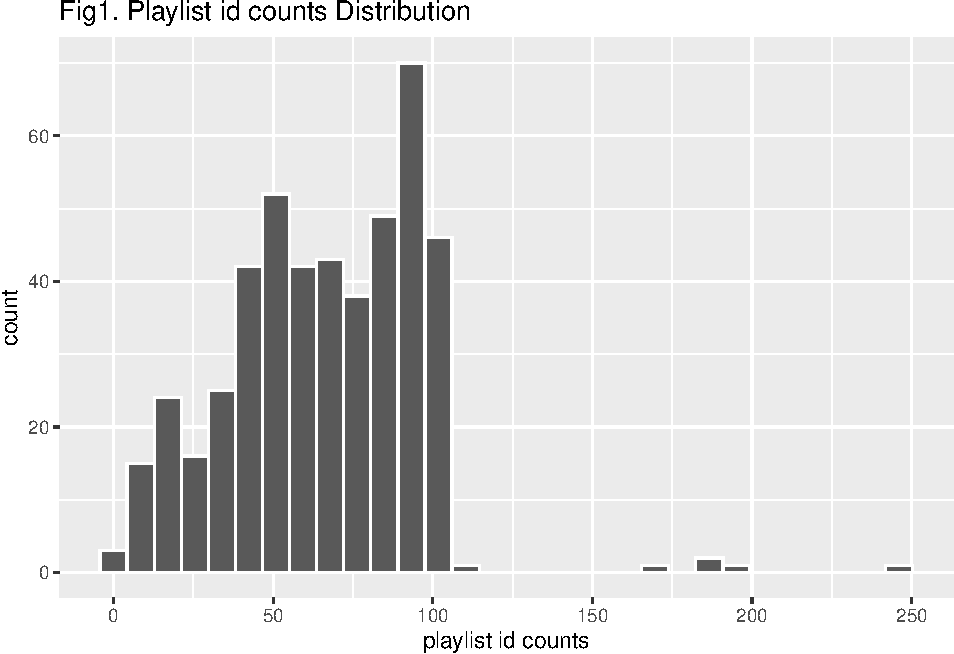
\includegraphics{Untitled_files/figure-latex/unnamed-chunk-8-1.pdf}

\begin{Shaded}
\begin{Highlighting}[]
\NormalTok{car\_tree\_tune }\OtherTok{\textless{}{-}} \FunctionTok{decision\_tree}\NormalTok{(}\AttributeTok{mode =} \StringTok{"classification"}\NormalTok{, }\AttributeTok{cost\_complexity =} \FunctionTok{tune}\NormalTok{()) }\SpecialCharTok{\%\textgreater{}\%} \FunctionTok{set\_engine}\NormalTok{(}\StringTok{"rpart"}\NormalTok{)}
\end{Highlighting}
\end{Shaded}

\begin{Shaded}
\begin{Highlighting}[]
\NormalTok{cost\_grid }\OtherTok{\textless{}{-}} \FunctionTok{grid\_regular}\NormalTok{( }\FunctionTok{cost\_complexity}\NormalTok{(), }\AttributeTok{levels =} \DecValTok{20}\NormalTok{ ) }
\NormalTok{cost\_grid}
\end{Highlighting}
\end{Shaded}

\begin{verbatim}
## # A tibble: 20 x 1
##    cost_complexity
##              <dbl>
##  1        1   e-10
##  2        2.98e-10
##  3        8.86e-10
##  4        2.64e- 9
##  5        7.85e- 9
##  6        2.34e- 8
##  7        6.95e- 8
##  8        2.07e- 7
##  9        6.16e- 7
## 10        1.83e- 6
## 11        5.46e- 6
## 12        1.62e- 5
## 13        4.83e- 5
## 14        1.44e- 4
## 15        4.28e- 4
## 16        1.27e- 3
## 17        3.79e- 3
## 18        1.13e- 2
## 19        3.36e- 2
## 20        1   e- 1
\end{verbatim}

\begin{Shaded}
\begin{Highlighting}[]
\NormalTok{doParallel}\SpecialCharTok{::}\FunctionTok{registerDoParallel}\NormalTok{()}
\NormalTok{tree\_tune }\OtherTok{\textless{}{-}} \FunctionTok{tune\_grid}\NormalTok{(}\AttributeTok{object =}\NormalTok{ car\_tree\_tune,}

\AttributeTok{preprocessor =} \FunctionTok{recipe}\NormalTok{(Sales\_high }\SpecialCharTok{\textasciitilde{}}\NormalTok{ ., }\AttributeTok{data =}\NormalTok{ car\_train), }\AttributeTok{resamples =}\NormalTok{ car\_cv, }\AttributeTok{grid =}\NormalTok{ cost\_grid)}
\end{Highlighting}
\end{Shaded}

\begin{Shaded}
\begin{Highlighting}[]
\FunctionTok{collect\_metrics}\NormalTok{(tree\_tune)}
\end{Highlighting}
\end{Shaded}

\begin{verbatim}
## # A tibble: 40 x 7
##    cost_complexity .metric  .estimator  mean     n std_err .config              
##              <dbl> <chr>    <chr>      <dbl> <int>   <dbl> <chr>                
##  1        1   e-10 accuracy binary     0.76      5  0.0256 Preprocessor1_Model01
##  2        1   e-10 roc_auc  binary     0.778     5  0.0244 Preprocessor1_Model01
##  3        2.98e-10 accuracy binary     0.76      5  0.0256 Preprocessor1_Model02
##  4        2.98e-10 roc_auc  binary     0.778     5  0.0244 Preprocessor1_Model02
##  5        8.86e-10 accuracy binary     0.76      5  0.0256 Preprocessor1_Model03
##  6        8.86e-10 roc_auc  binary     0.778     5  0.0244 Preprocessor1_Model03
##  7        2.64e- 9 accuracy binary     0.76      5  0.0256 Preprocessor1_Model04
##  8        2.64e- 9 roc_auc  binary     0.778     5  0.0244 Preprocessor1_Model04
##  9        7.85e- 9 accuracy binary     0.76      5  0.0256 Preprocessor1_Model05
## 10        7.85e- 9 roc_auc  binary     0.778     5  0.0244 Preprocessor1_Model05
## # ... with 30 more rows
\end{verbatim}

\begin{Shaded}
\begin{Highlighting}[]
\FunctionTok{collect\_metrics}\NormalTok{(tree\_tune) }\SpecialCharTok{\%\textgreater{}\%} \FunctionTok{filter}\NormalTok{(mean}\SpecialCharTok{==}\FunctionTok{max}\NormalTok{(mean))}
\end{Highlighting}
\end{Shaded}

\begin{verbatim}
## # A tibble: 1 x 7
##   cost_complexity .metric .estimator  mean     n std_err .config              
##             <dbl> <chr>   <chr>      <dbl> <int>   <dbl> <chr>                
## 1          0.0336 roc_auc binary     0.781     5  0.0195 Preprocessor1_Model19
\end{verbatim}

\begin{Shaded}
\begin{Highlighting}[]
\FunctionTok{select\_best}\NormalTok{( tree\_tune, }\StringTok{"roc\_auc"}\NormalTok{)}
\end{Highlighting}
\end{Shaded}

\begin{verbatim}
## # A tibble: 1 x 2
##   cost_complexity .config              
##             <dbl> <chr>                
## 1          0.0336 Preprocessor1_Model19
\end{verbatim}

\begin{Shaded}
\begin{Highlighting}[]
\NormalTok{best\_auc }\OtherTok{\textless{}{-}} \FunctionTok{select\_best}\NormalTok{( tree\_tune, }\StringTok{"roc\_auc"}\NormalTok{)}
\NormalTok{final\_spec }\OtherTok{\textless{}{-}} \FunctionTok{finalize\_model}\NormalTok{( car\_tree\_tune, best\_auc ) }
\NormalTok{final\_tree }\OtherTok{\textless{}{-}}\NormalTok{ final\_spec }\SpecialCharTok{\%\textgreater{}\%} \FunctionTok{fit}\NormalTok{( Sales\_high }\SpecialCharTok{\textasciitilde{}}\NormalTok{ . , }\AttributeTok{data =}\NormalTok{ car\_train )}

\FunctionTok{plot}\NormalTok{( final\_tree}\SpecialCharTok{$}\NormalTok{fit ) }
\FunctionTok{text}\NormalTok{( final\_tree}\SpecialCharTok{$}\NormalTok{fit )}
\end{Highlighting}
\end{Shaded}

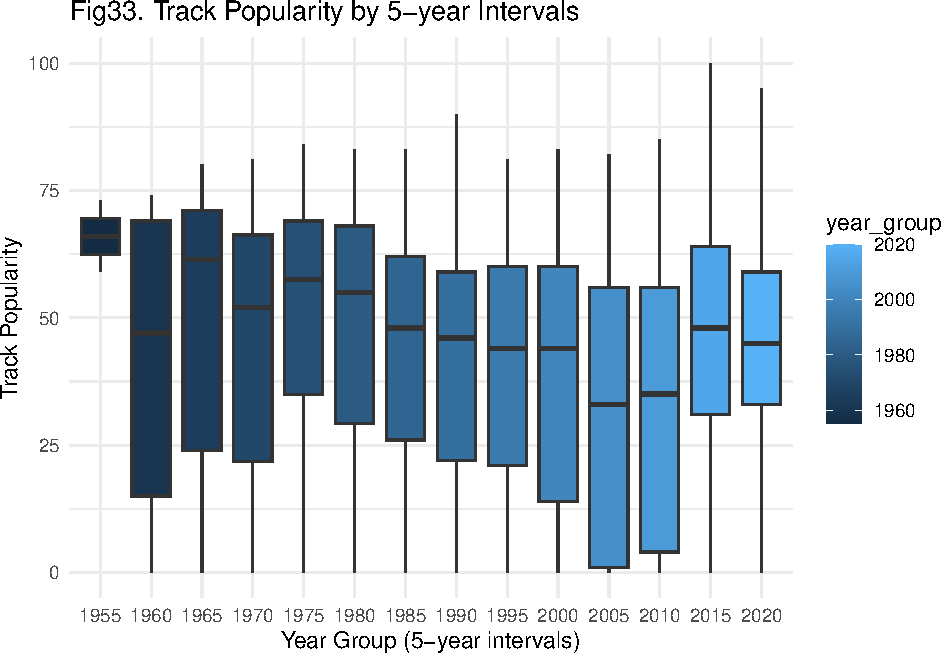
\includegraphics{Untitled_files/figure-latex/unnamed-chunk-15-1.pdf}

\begin{Shaded}
\begin{Highlighting}[]
\NormalTok{final\_tree }\SpecialCharTok{\%\textgreater{}\%} \FunctionTok{vip}\NormalTok{()}
\end{Highlighting}
\end{Shaded}

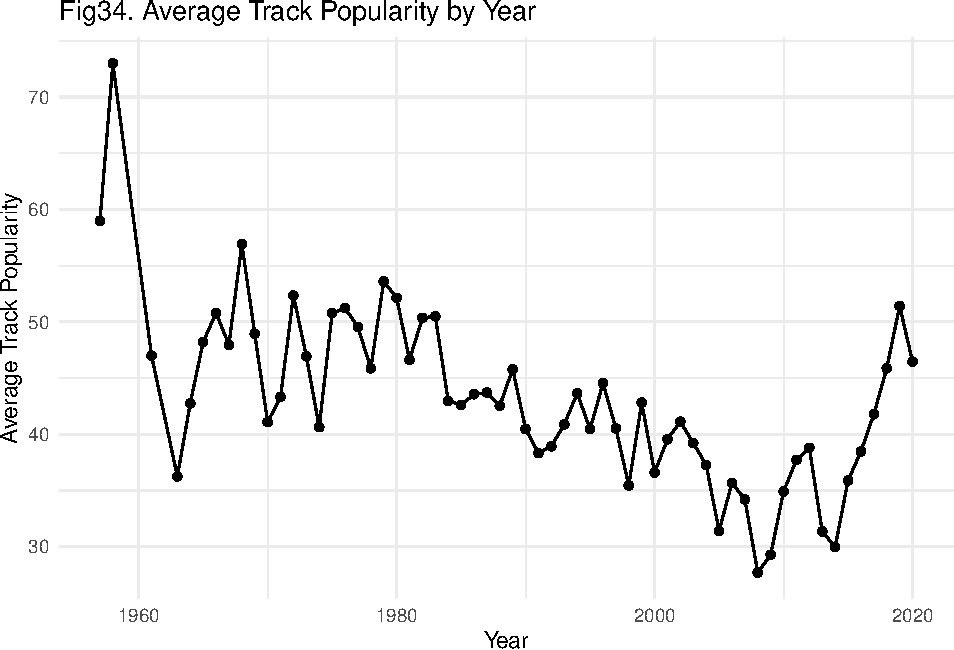
\includegraphics{Untitled_files/figure-latex/unnamed-chunk-16-1.pdf}

\begin{Shaded}
\begin{Highlighting}[]
\NormalTok{car\_train\_preds }\OtherTok{\textless{}{-}}\NormalTok{ car\_tree }\SpecialCharTok{\%\textgreater{}\%}

\FunctionTok{predict}\NormalTok{( }\AttributeTok{new\_data =}\NormalTok{ car\_test,}\AttributeTok{type =} \StringTok{"class"}\NormalTok{) }\SpecialCharTok{\%\textgreater{}\%} \FunctionTok{bind\_cols}\NormalTok{( car\_test )}

\NormalTok{car\_train\_preds }\SpecialCharTok{\%\textgreater{}\%} \FunctionTok{metrics}\NormalTok{( }\AttributeTok{truth =}\NormalTok{ Sales\_high, }\AttributeTok{estimate =}\NormalTok{ .pred\_class)}
\end{Highlighting}
\end{Shaded}

\begin{verbatim}
## # A tibble: 2 x 3
##   .metric  .estimator .estimate
##   <chr>    <chr>          <dbl>
## 1 accuracy binary         0.71 
## 2 kap      binary         0.401
\end{verbatim}

\begin{Shaded}
\begin{Highlighting}[]
\NormalTok{car\_preds }\OtherTok{\textless{}{-}} \FunctionTok{predict}\NormalTok{( final\_tree, }\CommentTok{\# Get probability predict }
                      \AttributeTok{new\_data =}\NormalTok{ car\_test,}

\AttributeTok{type =} \StringTok{"prob"}\NormalTok{ ) }\SpecialCharTok{\%\textgreater{}\%}

\FunctionTok{bind\_cols}\NormalTok{( car\_test }\SpecialCharTok{\%\textgreater{}\%} \CommentTok{\# Add on the truth.}
  \FunctionTok{select}\NormalTok{( Sales\_high ) }\SpecialCharTok{\%\textgreater{}\%} 
    \FunctionTok{mutate}\NormalTok{( }\AttributeTok{model =} \StringTok{"Tuned"}\NormalTok{ ) ) }\SpecialCharTok{\%\textgreater{}\%} \CommentTok{\# Add a vari }
\FunctionTok{bind\_rows}\NormalTok{( }\CommentTok{\# Bind on the predictions from the orginal tre }
  \FunctionTok{predict}\NormalTok{( car\_tree, }\CommentTok{\# Get probability predictions }
           \AttributeTok{new\_data =}\NormalTok{ car\_test,}
            \AttributeTok{type =} \StringTok{"prob"}\NormalTok{ ) }\SpecialCharTok{\%\textgreater{}\%}

  \FunctionTok{bind\_cols}\NormalTok{( car\_test }\SpecialCharTok{\%\textgreater{}\%} \CommentTok{\# Add truth and model tacker }
               \FunctionTok{select}\NormalTok{( Sales\_high ) }\SpecialCharTok{\%\textgreater{}\%}

    \FunctionTok{mutate}\NormalTok{( }\AttributeTok{model =} \StringTok{"Untuned"}\NormalTok{ ) )}

\NormalTok{) }
\NormalTok{car\_preds }\SpecialCharTok{\%\textgreater{}\%} \FunctionTok{group\_by}\NormalTok{( model ) }\SpecialCharTok{\%\textgreater{}\%} \CommentTok{\# Seperate by model type. }
  \FunctionTok{roc\_curve}\NormalTok{( }\AttributeTok{truth =}\NormalTok{ Sales\_high, }\AttributeTok{estimate =}\NormalTok{ .pred\_No ) }\SpecialCharTok{\%\textgreater{}\%}\NormalTok{ autoplot}
\end{Highlighting}
\end{Shaded}

\begin{verbatim}
## Warning: Returning more (or less) than 1 row per `summarise()` group was deprecated in
## dplyr 1.1.0.
## i Please use `reframe()` instead.
## i When switching from `summarise()` to `reframe()`, remember that `reframe()`
##   always returns an ungrouped data frame and adjust accordingly.
## i The deprecated feature was likely used in the yardstick package.
##   Please report the issue at <]8;;https://github.com/tidymodels/yardstick/issueshttps://github.com/tidymodels/yardstick/issues]8;;>.
\end{verbatim}

\includegraphics{Untitled_files/figure-latex/unnamed-chunk-18-1.pdf}

\begin{Shaded}
\begin{Highlighting}[]
\NormalTok{Gini\_left}\OtherTok{=}\FloatTok{0.30}\SpecialCharTok{*}\FloatTok{0.70} \SpecialCharTok{+} \FloatTok{0.70}\SpecialCharTok{*}\FloatTok{0.30}

\NormalTok{Gini\_left}
\end{Highlighting}
\end{Shaded}

\begin{verbatim}
## [1] 0.42
\end{verbatim}

\begin{Shaded}
\begin{Highlighting}[]
\NormalTok{Gini\_right}\OtherTok{=}\FloatTok{0.74}\SpecialCharTok{*}\FloatTok{0.26} \SpecialCharTok{+} \FloatTok{0.26}\SpecialCharTok{*}\FloatTok{0.74}

\NormalTok{Gini\_right}
\end{Highlighting}
\end{Shaded}

\begin{verbatim}
## [1] 0.3848
\end{verbatim}

\begin{Shaded}
\begin{Highlighting}[]
\NormalTok{Weighted\_gini}\OtherTok{=}\FloatTok{0.78}\SpecialCharTok{*}\NormalTok{Gini\_left}\FloatTok{+0.22}\SpecialCharTok{*}\NormalTok{Gini\_right }
\NormalTok{Weighted\_gini}
\end{Highlighting}
\end{Shaded}

\begin{verbatim}
## [1] 0.412256
\end{verbatim}

\end{document}
